% ATENÇÃO - veja com o seu orientador se você vai ter este capítulo e se este vai ter nome!
\chapter{Metodologia}
\label{cap:metodologia}

\begin{itemize}
    \item RQ1: How often do breaking changes manifest in the client package?
\end{itemize}

A stack trace is a report that provides information about program subroutines. It is commonly used for certain kinds of debugging, where a stack trace can help software engineers figure out where a problem lies or how various subroutines work together during execution. When \textit{npm install} or \textit{npm test} results in an error, it raises a stack trace. All information about the error and the calls to providers are shown in the stack trace. Figure \ref{fig:trace} shows a generic example of a stack trace of one error.

\begin{figure}
    \centering
    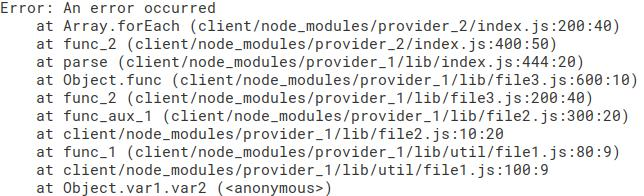
\includegraphics[scale=0.7]{figuras/stack_trace.jpeg}
    \caption{Generic stack-trace}
    \label{fig:trace}
\end{figure}{}

The stack trace is the base to analyze and an error.
All releases of any package that broke in the \textit{npm install} or \textit{npm test} were analyzed manually. The first step to analyze an error is differentiated between an error that wasn't caused by any provider, which is an error that occurred exclusively in the client package where the providers didn’t influence, and a breaking change error, that the errors occurred in provider package and it broke a client. There are two ways to conduct this step.

The first way is to take a look at the stack trace of the error and verify the calls to providers. When in the stack trace there isn't called to any providers, the error probably doesn’t refer a breaking change, because any provider was called in this error. So, the error is in the client code. To confirm this, the next commit in GitHub, after the release of the client, is verified. The objective is to verify if the error was fixed in any client commit. If true, the error is confirmed as a non-breaking change.
Some types of errors can be resolved in the code of the client. This error isn’t breaking change. Errors like \textit{SyntaxError} and \textit{ReferenceError}, where the client wrote the wrong code. Example:

\begin{lstlisting}[style=Javascript, label=cod:syntax:error, caption={Reference Error code in JavaScript}]
const a = 0 = 0;
\end{lstlisting}


In these errors, the npm raises a \textit{ReferenceError}. If the error is in the client code, nor is it necessary to look at \textit{GitHub}, because, for sure, the error is a non-breaking change. So, the code was fixed and the \textit{npm install} or \textit{npm test} is executed again to verify if any other error appeared.

The second way is when the errors can be a breaking change. This often occurs when the stack trace contains calls to any providers. However, providers like \textit{Mocha, Istanbul, Jasmine} and so on, that is, test frameworks, and task runners, like \textit{Grunt}, it is shown in stack trace but usually has no errors, because they only execute the files to test/tasks. So, when one of these providers is at the bottom of the stack tracer, they just called/execute the files/providers that contain the errors. Then, there’s a high probability that this error is a breaking change and this error can be caused by any provider.
To confirm this, the best place is in the \textit{GitHub}. The repository of the package contains all the information about the development. There are many ways to retrieve information. The easiest and most reliable way is to verify in a changelog file. These files, in general, are the \textit{CHANGELOG.md}, \textit{HISTORY.md} and others like this. These files contain the description of all changes about all packages releases. And many breaking changes are described there. For example, the release 5.0.0 of \textit{Mocha} contains a breaking change and was documented in \textit{CHANGELOG.md}. Figure \ref{fig:bc_documentation} show this documentation.

\begin{figure}
    \centering
    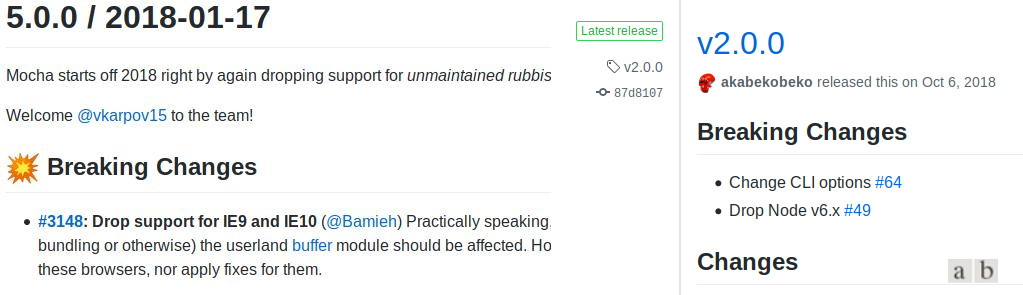
\includegraphics[scale=0.55]{figuras/bc_documentation.jpeg}
    \caption{Breaking Change documentation in README}
    \label{fig:bc_documentation}
\end{figure}{}

Other types of changelogs are the release notes. These are found in the comments of release. However, many and many repositories don’t contain a changelog file. Then, the next step is the search for any issue that contains some information about the error. In general, the issues contain much information, because of the developers and the owners of the package comment about the error. And more, many related issues are linked, increasing the number of information. Also, pull request works in the same way as issues.

Another important way is to install another release of the provider. So, it's possible to find out from which release the error started or which release the error was fixed. Also, there are other ways to verify if the error is in the provider. This is, compare the diff code between two provider releases; verify the provider commits; and change provider code.
The Figure \ref{fig:step_analyze} show a summary of these steps.

\begin{figure}
    \centering
    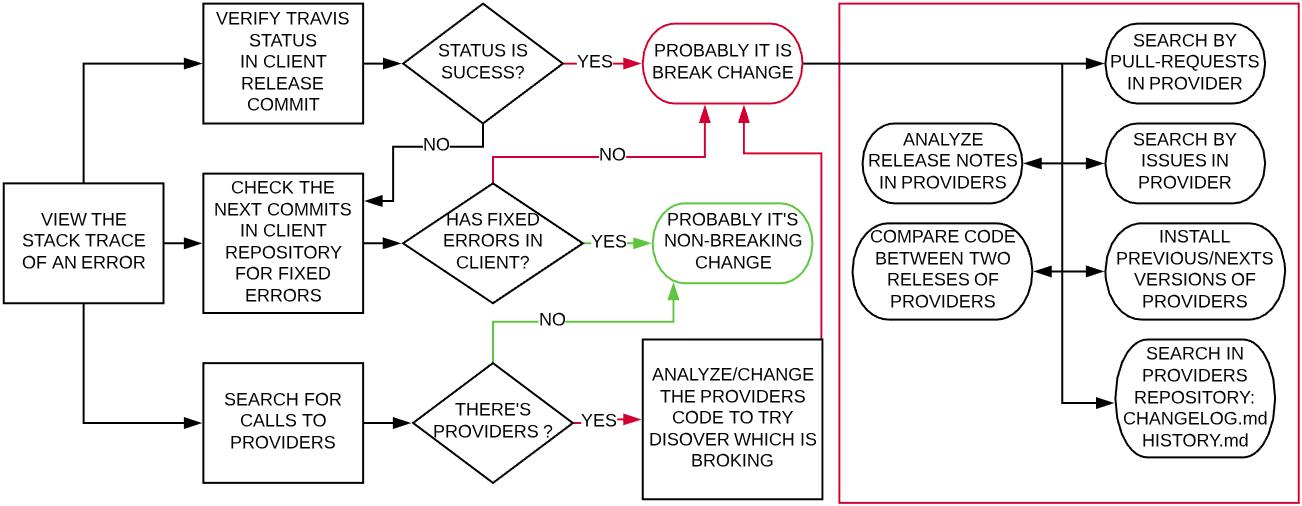
\includegraphics[scale=0.35]{figuras/step_analyze.jpeg}
    \caption{Steps to analyze an error}
    \label{fig:step_analyze}
\end{figure}
Some integrated systems can help to discover breaking changes. These systems are \textit{Travis, Jenkins, Codeship, CircleCI} and so on, and store the results of the npm install and npm test in the moment of a commit. It can help in the following way: if in the commit of a release the status of npm install or npm test was a success, and now is an error, then it occurred by a provider because the code of client is the same in the working tree and only the provider code was updated. However, just some of the sorted packages contain an integrated system.

Another detail is the packages that connect with some type of service likes, \textit{MySql, CouchDB, Redis} and so on. From all 385 packages, x required one of these services. When the \textit{npm install} or \textit{npm test} raises an error because of the connection, in manual analyze the required services were ability and re-executed the package. So, if the error was persister because the connection, the package was classified was \textit{Undiscovered Error}.

So, from all release analyze was saved many informations:

\begin{enumerate}
    \item Documentation about the error: issue, changelog, pull-request and so on;
    \item Who fixed the error: client or provider;
    \item How long did the error take to get fixed;
    \item Fixed in major, minor or patch; and
    \item In how many releases the error existed.
\end{enumerate}{}

Nor all information may be recovered. For example, if an error wasn’t fixed, then neither the client nor the provider repaired the error.

\begin{itemize}
    \item RQ2: What issues in the provider package cause the manifestation of a breaking change?
\end{itemize}

For each error in \textit{npm install} or \textit{npm test}, it was manually analyzed. The objective is to do a grouping of similar errors and categorize then. For example, Figure \ref{fig:error_category} shows two errors in which one a function was renamed and the client tries to access the previous name.

\begin{figure}[!h]
    \centering
    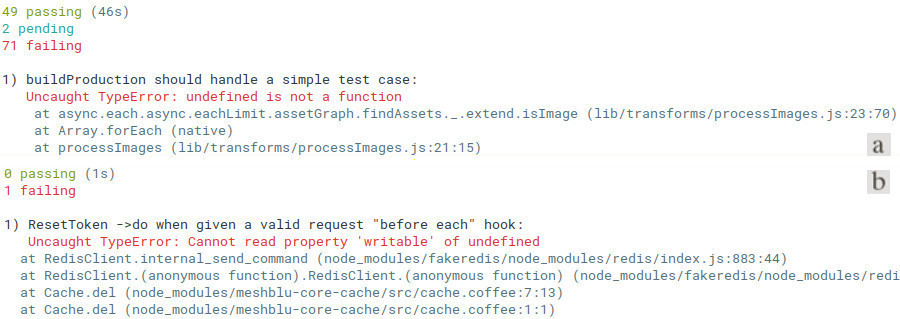
\includegraphics[scale=0.5]{figuras/error_category.jpeg}
    \caption{Two error caused by a renamed function}
    \label{fig:error_category}
\end{figure}

The first error in the Figure \ref{fig:error_category} is 

\begin{itemize}
    \item RQ3: How do client packages recover from the manifestation of breaking change?
\end{itemize}

Since the customer recovers from the error, there are two ways to know how it recoverer. The first way is when the provider fixes his code and the client just updates the string of versioning in \textit{package.json}, if it needs. To the provider fixes the error, one issue may be done in his repository. The second way is when the client must do some work to fix the code. In this case, the client can fix the provider code and do a pull-request or change his code to work with the provider. And of course, may have cases that anyone does nothing. There is a breaking change and it’s never been fixed.

Where information about this RQ is retrieved is \textit{GitHub}. This information can be found at \textit{CHANGELOG, release-notes, issues,} and \textit{pull-requests}. If the \textit{changelog} contains information about fixed errors, in general, the related \textit{issues} are marked. From these \textit{issues}, a lot of more information can be recovered, like \textit{pull-requests} that are also marked in the \textit{issue}, other \textit{issues}, commentaries and more. All of this information can help us to discover which one -- client or provider -- fixed the \textit{breaking change} and how it was fixed.

\textit{Commits} are the alternative to \textit{issues} when the search is in the client repository. The \textit{commits} contain all changes in files and the all updates providers in \textit{package.json}. Commits message like \textit{update dependencies, fix dependencies, fix errors} an so on, suggests that something about any dependencies was fixed. This information is very important, because, since the provider was fixed and the client just updates it, the commit messages can tell the reason for this update - or downgrade.

%---------------------------------------------------%
\section{Considerações Finais}
\label{cap:metodologia:sec:consideracoes:finais}

Esta é uma sugestão de seção para dar um fechamento em cada uma dos capítulos.

(ATENÇÃO - veja com o seu orientador se é uma seção necessária (pois trate-se de estilo de escrita))